\documentclass[conference]{IEEEtran}

\usepackage{amssymb,amsmath,epsfig,graphics,enumerate,float,subfigure,verbatim,url,multirow,caption}
\usepackage[usenames,dvipsnames]{color}
\usepackage[vlined,ruled]{algorithm2e}
\usepackage{tikz,alltt,arydshln,longtable,listings,bm}
\usepackage{listings}
\usepackage{caption}
\usepackage{graphicx}
%\usepackage{float}
 
%\newcommand{\comment}[1]{} 
\newcommand{\etc} {\emph{etc.}}
\newcommand{\etal}{\emph{et~al. \/}}
\newcommand{\eg}  {\emph{e.g., \/}}
\newcommand{\ie}  {\emph{i.e., \/}}
\def\Reals{\mathbf{R}}
\def\Ints{\mathbf{Z}}
\def\Nats{\mathbf{N}}
\def\E{\mathbb{E}}
\def\P{\mathbb{P}}
\def\A{{\cal A}}
\def\bf{\bfseries}
\newcommand{\nop}[1]{}
\newcommand{\from}[2]{{\bf [{\sc from #1:} #2]}}
\newcommand{\ra}{\mbox{$\rightarrow\;$}}
\newcommand{\rax}{\mbox{$\;\rightarrow\;$}}
\newcommand{\lb}{\mbox{$\langle$}}
\newcommand{\rb}{\mbox{$\rangle$}}
\newcommand{\cln}{\mbox{$:$}}
\newcommand{\crossdouble}{\makebox[2.85ex]{\bf ---}\makebox[-2.95ex]{}}
\newcommand{\st}{\mbox{$\ast$}}
\def\ssp{\mbox{\hspace*{2.5ex}}}
\def\sp{\mbox{\hspace*{6.5ex}}}
\def\Bsp{\mbox{\hspace*{30ex}}}
\def\dq{\mbox{''}}
\def\cod{\mbox{$~:-~$}}
\def\parag{{\vspace{0.01in} }}
\def\boxend{\hspace*{\fill} $\blacksquare$}
\def\qed{\hspace*{\fill} $\blackbox$}
%\def\QED{\mbox{\rule[0pt]{1.5ex}{1.5ex}}}
\def\proof{\noindent\hspace{2em}{{\itshape Proof: }}}
\def\endproof{\hspace*{\fill}~\qed\par\endtrivlist\unskip}

\begin{document}
\title{CASCADES: Modeling and Simulation of Cyber Attacker Behaviors for Network Threat Analysis\
\vspace*{-20pt}}

\author{\textsuperscript{1}Stephen Moskal, \textsuperscript{2}Michael Kuhl, \textsuperscript{1}Shanchieh Jay Yang \\
%\IEEEauthorblockN{Stephen Moskal}
%Department of Computer Engineering\\
\textsuperscript{1}Department of Computer Engineering, \textsuperscript{2}Department of Industrial Systems and Engineering\\
Rochester Institute of Technology, Rochester, New York 14623\\
\{sfm5015, mekeie, jay.yang\}@rit.edu
}
\maketitle

\section{Introduction}
\label{sec:intro}

Recent high-profile data breaches has caused a shift in the cyber security field to focus more on prevention of cyber attacks as opposed to detection of threats.  Security assessments of enterprise computer networks by the use of vulnerability assessment tools and penetration tests are now common and in most cases a requirement.  Despite these prevention techniques, recent data breaches are causing billions of dollars of losses to companies as current techniques are not capable of exposing all issues in a network.  The complexity of this problem is the result of the size a network and the sheer number of configurations possible along with the diverse skills and attack preferences of the adversaries.  Static network analysis that uses attack graphs, \eg \cite{jha2002two, sheyner2002automated, kotenko2014security, kotenko2015capec} exhaustively exposes attack paths but struggles to provide realistic attack scenario representation because only vulnerability data is used.  Game Theory (\cite{wang2010network, chung2016game}) and Agent-based (\cite{kotenko2005agent,grunewald2011agent}) modeling techniques were applied to this application to capture how the attacker interacts with the network but where not flexible in the types of attacks that could be modeled.  Simulation has been applied to the cyber domain (\cite{grunewald2011agent, moskal2013simulating,moskal2014context}) and is a promising technique, however due to the complexity of the problem it is difficult to achieve realistic simulations.  This work expands on \cite{moskal2014context} by developing a cyber attack simulator that identifies key aspects of computer networks and cyber attack behaviors to provide a realistic simulation while reducing the model complexity.  

CASCADES (Cyber Attack Scenario and Network Defense Simulator) is a cyber attack scenario simulation platform that exposes the relationship and dependency of the cyber attacker's behaviors to the physical network configuration.   By modeling both the network and the attacker it is possible to understand how an attacker effects a network but also how a network configuration effects the attacker's progress given an attack scenario.  CASCADES employs a knowledge-based behavior model \cite{moskal2016knowledge} representing the capabilities, opportunities, intent, and preferences of the individual attacker to aid in the understanding of the key information the attacker needed to make decisions as the attack progresses.   By representing the attacker based on the knowledge developed throughout an attack and how the attacker uses that information along with the integration of the Cyber Attack Kill Chain, CASCADES provides the capability of representing a wide variety of attackers while still maintaining realistic attack scenarios.  This allows the generation of many attack graphs while maintaining accuracy along with understanding the interplay between the attacker and the defender without requiring an expert to configure.  Preliminary results of CASCADES shows both the types of attackers play a large role in how resilient an network is to an attack but also the effects of how a misconfigured network has on the attacker's progress. 

%This complexity was realized in \cite{jha2002two, sheyner2002automated} where attack graphs where generated based only on the vulnerabilities on a network resulting in graphs of thousands of nodes and tens of thousands of edges for unrealistically small networks (4-5 machines) and few attack types.  The attack graphs generated where exhaustive and required an expert to filter out the realistic attack paths.  This was then optimized by \cite{xie2010using} to take in account real-world attack scenario information from National Vulnerability Database (NVD) to give some context of actual cyber attack scenarios and then later Common Attack Pattern Enumeration and Classification (CAPEC) was applied to attack graphs by \cite{kotenko2014security, kotenko2015capec} to achieve even more realistic attack scenarios.  However each of these methods to not take in consideration the personalities and intricacies of the individual cyber attackers.

\section{Context Models for Simulation}
CASCADES is a multithreaded model-driven cyber attack simulator built off the previous efforts of MASS in \cite{moskal2014context}.  CASCADES uses 4 major context models: Virtual Terrain (VT), the Vulnerability Database, Attacker Behavior Model (ABM), Intent Module.   The VT is the description of the physical network consisting of routers, machines, and the connections between them.  This also contains the services that are installed on the machines which describes the vulnerabilities.  All vulnerability data is stored in the Vulnerability Database which is a preparatory database consisting of data from NVD, MITRE, Snort, etc.  

A critical component of CASCADES is the ABM which houses the logic to select the actions performed by the attacker.  The ABM uses the network knowledge gained from performing reconnaissance or previously attempted attack actions to influence the type of attack the attacker may choose along with the preference the attacker may have on certain types of targets or actions.  Tightly coupled with the ABM, the intent module describes the goals or the intentions of the attacker for the simulation.   The intent can be described as generically to attack a certain type of machine (\eg customer information database) or strictly ``if... then" intentions to provide more robust and reactionary intents.  Other context models are also defined in CASCADES including: moving target defenses (MTD), intrusion detection systems (IDS), and the noise generator (generates normal network traffic).  Figure \ref{fig:overview} shows the overall system architecture of CASCADES.

\begin{figure}[htbp]
	\centering
	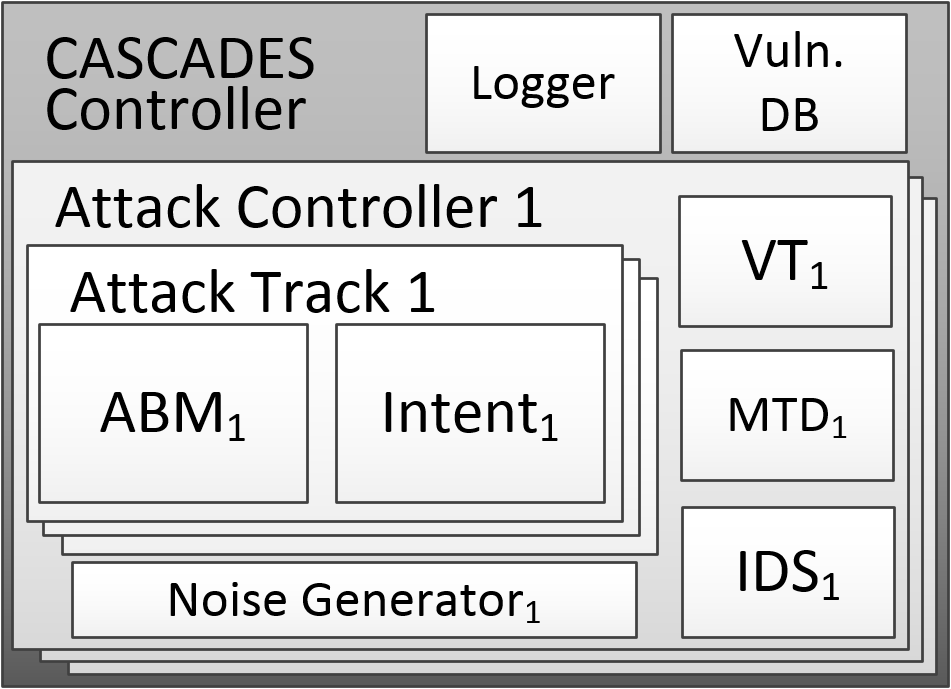
\includegraphics[width=6cm,keepaspectratio]{Figure_Overview.png}
	\caption{The overall CASCADES system architecture}
	\label{fig:overview}
\end{figure}

\section{Experiments and Analysis}
A test network is set up with 16 machines modeled with key aspects commonly found in enterprise networks like DMZ's, guest networks, administrative machines, and high security subnets. For these simulations, the intent of the attacker was to exfiltrate information contained on the backup server located in the deepest part of the network.  For these experiments, three different types of attackers were modeled: an amateur, an expert, and a random attacker. The amateur attacker has a limited skill set, is not concerned with being caught, and gives up easily upon failure.  The expert attacker is methodical in the types of targets they choose and uses stealthy attack actions.  Whereas the random attacker is a brute force attacker that literally randomly selects actions which is used as a worst case baseline.  For comparison, the three attackers are simulated on the base network as well as a misconfigured network with a firewall misconfiguration exposing a secured machine to the internet to demonstrate how the network configuration effects the attacker's progress.  Each case and attacker is simulated 1000 times to measure the variance between simulations.  Figure \ref{fig:network} shows an example of a single simulated step of an attack path using the CASCADES UI.

\begin{figure}[htbp]
	\centering
	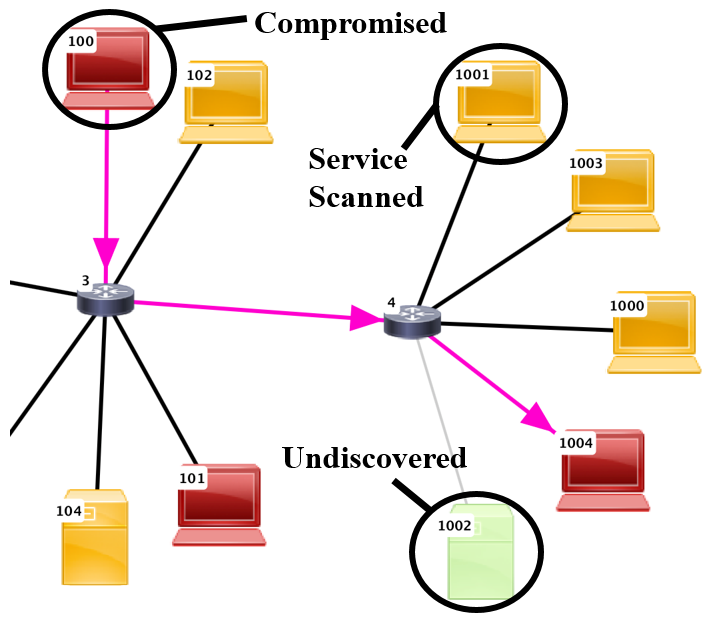
\includegraphics[width=6cm,keepaspectratio]{NetworkDiagram2.png}
	\caption{A partial simulated attack path on a network showing the state of the affected machines.}
	\label{fig:network}
\end{figure}

Table \ref{steps} shows the number of actions taken to achieve the intent and the failure rate (percent of time the attacker failed to achieve their intent) for both of the networks and the three attackers.   In the case of the base network, both the amateur and expert attacker took the same average amount of steps to complete their intent.  This is due to the amateur attacker having the necessary skills to penetrate the network along with the network being small enough that the amateur could find the goal machine.  However, the amateur failed to achieve their intent 17.8\% of the time on the base network compared to the 1.8\% of the expert.   When analyzing the misconfigured network the number of actions performed for both the expert and the random attacker decreased significantly while the amateur increased slightly.  This is because the amateur did not have the skills to successfully take advantage of this newly introduced security hole in the network.  It can also be seen that with this misconfiguration the naive random attacker is approaching the average number of steps that the amateur attacker, which is concerning from an analysis perspective because even the brute force case is performing well incomparison.

\begin{table}[]
\centering
\caption{Simulation statistics for both network types and the three attackers.}
\label{steps}
\begin{tabular}{|cc|ccc|}
\hline
\begin{tabular}[c]{@{}c@{}}Network\\ Config.\end{tabular} &              & Amateur & Expert & Random \\ \hline
\multirow{2}{*}{Base}                                     & Avg. Steps   & 27.5    & 27.6   & 47.4   \\
                                                          & Failure Rate & 17.8    & 1.8    & 0      \\ \hline
\multirow{2}{*}{Error}                                    & Avg. Steps   & 28.8    & 20.4   & 33.5   \\
                                                          & Failure Rate & 15.5    & 1.2    & 0   \\ \hline
\end{tabular}
\end{table}

\section{Lessons Learned \& Conclusions}
\label{sec:concl}
The test example shown in this abstract demonstrates the capability to analyze various different types of attackers in different situations by evaluating the knowledge the attacker gains throughout an attack scenario.  CASCADES has additional capabilities such as exposing critical weaknesses in a network based on the frequency of attacks on a particular machine or the frequency a service or vulnerability is attempted and a fully functional UI for analysis of attacks.  We learned that by modeling the attacker's decisions based off of the knowledge gained throughout an attack and applying a Cyber Attack Kill Chain to the simulation, simulation is viable and promising approach to network threat analysis.  The results of this work also emphasized the complexity of a cyber attack and what makes each cyber attacker different from one another.  From this work we have a better understanding of what are the parameters needed to represent cyber attacker behaviors and knowledge and we can refine and add new parameters to better model behaviors which then provides better analysis of network threat resilience.  

%While the knowledge-based model is a promising concept, it does not come without faults.  For example, the behavior models themselves are flexible in their description and can model many different types of attackers, it is still time consuming to develop the model accurately and requires extensive trial and error to configure properly.  Likewise, the parameters that are available to the user to configure the ABM can be expanded on to provide better control over the simulation.  Currently the parameters are based upon the number of service scanned machines or compromised machines for example and not features pertaining to the types of machines or information on the machines. 

\bibliographystyle{IEEETran}
\bibliography{rit-thesis}

\end{document}
